% Requires graphicx. Place the PDF alongside the manuscript or on \graphicspath.
% Single-column float in a two-column manuscript.
\begin{figure}[t]
    \centering
    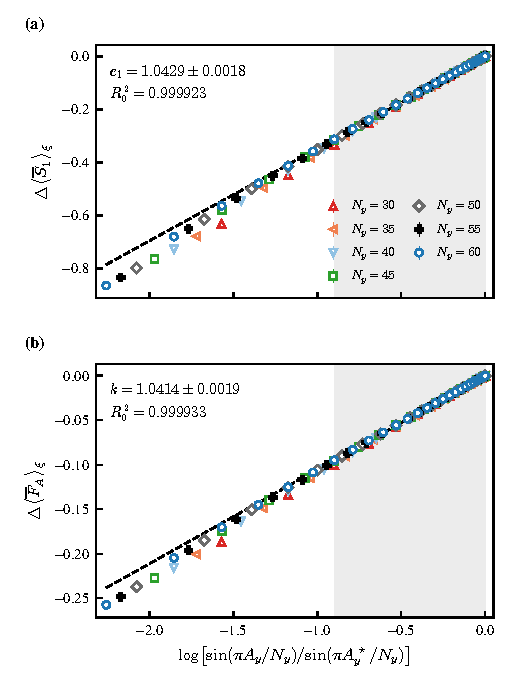
\includegraphics[width=\columnwidth]{endpoint_entropy_charge_mean_curve_collapse_2x1.pdf}
    \caption{\textbf{Trajectory-averaged entropy and charge-variance collapse.}
    (a) Von Neumann entropy and (b) intrinsic subsystem charge variance for
    hard-wall circuits at $N_x=20$, $N_y=30,35,\ldots,60$, and $t=2N_y$,
    starting from pure half-filled random states. At each size, periodic strip
    origins are averaged within each of $S=100$ independent trajectories,
    followed by the trajectory average before fitting.
    Curves are anchored at $A_y^\star=\lfloor N_y/2\rfloor$ by subtracting
    their half-strip values; the horizontal coordinate is
    $\Delta X=\log[\sin(\pi A_y/N_y)/\sin(\pi A_y^\star/N_y)]$.
    Points at $A_y=1$ are omitted. Black dashed lines show joint through-origin fits over
    $A_y=8,\ldots,A_y^\star$ with equal total weight per size, yielding
    $c_1=3m_S$ and $k=\pi^2m_F$. Gray shading spans the combined fit domain.
    Bars show ordinary trajectory SEMs; coefficient errors retain the full
    covariance across strip widths.}
    \label{fig:entropy-charge-mean-collapse}
\end{figure}
